% Begin
\documentclass[12pt]{article}

% Packages
\usepackage[top=2cm, bottom=3cm, left = 1in, right = 1in]{geometry}
\usepackage[fleqn]{amsmath}
\usepackage{amssymb}
\usepackage{anysize}
\usepackage{graphicx}
\usepackage{subcaption}
\usepackage{float}
\usepackage{comment}
\usepackage{multirow}
\usepackage{xcolor}
\usepackage[
	backend=biber,
	maxcitenames=2,
	maxbibnames=10,
	citestyle=authoryear,
	bibstyle=authoryear,
	isbn=false,
	url=false,
	doi=false]{biblatex}
\renewbibmacro{in:}{}
\captionsetup[subfigure]{labelformat=empty}

% Bib file
\addbibresource{bibfile.bib}

% Paper style
\geometry{a4paper}

% Equation (section.equation)
\numberwithin{equation}{section}

% Title
\title{Report on An Urban Truck Scheduling and Routing Problem}
\author{Zefeng Lyu, Rui Zhou, Zeyu Liu}
\date{}

% Begin Document
\begin{document}

%MakeTitle
\maketitle

%Introduction
\section{Introduction}

	\paragraph{}Nowadays, electronic commerce offers us a new way for shopping and plays an increasingly important role in people’s daily life. Many electronic commerce companies, such as Amazon, Alibaba or Jing Dong have become famous all around the world. In order to satisfy customer demands and reduce transportation costs, establishing efficient and economic logistic systems is significantly crucial. 
	
	\paragraph{}The Urban truck scheduling and routing problem talked in this article is a classic vehicle routing problem (VRP), which seeks to find routs to deliver goods from a central depot to a set of geographically dispersed customers \parencite{Coelho2016}. There exists a wide variety of VRPs and a broad literature on this class of problems \parencite{Laporte1992}. We could get a new VRP if only we change the side conditions, such as capacity restrictions, time windows, etc. It is notable that electric vehicles become more and more popular because of their property of environment-friendly and economic \parencite{Hiermann2016}. When electric vehicles are involved, problem will become more complicated because we need to determine whether a vehicle should get charged and move further or just turn back. When electronic vehicle is engaged, determining the time and station for recharging is crucial \parencite{Zhang2018}. Besides, some researchers pay more attention to our environment protection. Bektas and Laporte (2011) are the first to propose the Pollution-Routing Problem (PRP) to offer insights into environment-friendly vehicle routing. \parencite{Lin2014} upgraded the traditional objective to minimizing system-wide costs related to economic and environmental issues.
	
	\paragraph{}In this article, we study a real CVRPTW problem involving a distribution center of an electronic commerce company in China that serves 1000 customers. In this case, fixed, variable (transportation) and waiting cost need to be considered and minimized. A few constraints of this version VRP are listed as follows. 
	
	\begin{itemize}
		\item Capacity: Each vehicle has an identical volume and weight limitation.
		
		\item Time Window: Vehicles are supposed to arrive in the time windows. But early arrival is allowed at the cost of waiting.
		
		\item Distance range: limited by the energy, each truck has a maximum traveling distance. 
	\end{itemize}

	\paragraph{}We solve this problem by using heuristic algorithm and simulation. Heuristic algorithms for the VRP can often be derived from procedures derived from the TSP \parencite{Laporte1992}. There are lots of heuristic algorithms, such as Clarke and Wright algorithm, Tabu search algorithm, Genetic algorithm, Particle swarm algorithm, etc. However, when applying these methods to VRPS, care must be taken to ensure that only feasible vehicle routs are created \parencite{Laporte1992}. Simulation software is another helpful tool for VRP problem. AnyLogic, one of the most popular simulation software, can be used in to strengthen the model by introducing random traffic flow to simulate practical traffic conditions \parencite{Fan2009}. Besides, AnyLogic could visualize the result and make it readable for non-technical personnel.
	
	\paragraph{}The rest of this article is organized as follows. Section 2 defines the problem and proposes a mathematical model. Section 3 introduces input data and algorithms used to solve the problem. Section 4 demonstrates how AnyLogic is employed to create a simulation model to visualize the solutions. Finally, we draw a conclusion and give out some future research we may do in Section 5.


% Problem statement
\section{Problem \& Model}

	\paragraph{}We are looking at a distribution center in Beijing, China owned by Jing Dong (JD), a Chinese company engaged in electronic commerce as well as logistics. This center provides package delivery services to over a thousand customers around the city. The company is trying to find out how many trucks are needed and what routes should each truck take to achieve a minimal delivery cost and satisfy all customer demands. Each customer expects the delivery to arrive before 8 pm in the evening. Late deliveries incurs a penalty cost of 24 yuan per hour. Each truck can serve multiply customers but each customer could only be served by one truck at one time. Besides, the capacity of trucks should be taken into consideration when it serve multiply customers. The objective is to determine the number of trucks to be used and design their routes so that the total cost, including fixed cost (of trucks), transportation cost and waiting cost, is minimized. Additionally, the problem adopts following assumptions:

	\begin{itemize}
	\item The trucks begin at the distribution center and need to return to the distribution center once packages are delivered;
	\item The unloading time for each customer is a constant of 0.5 hour.
	\item The coefficient of waiting cost described is 24 yuan/h. Later arrival is not allowable.
	\end{itemize}
	
	\paragraph{}We model this problem as a Vehicle Routing Problem with Time Windows and Capacity Constraints (VRPTWCC)\parencite{Schneider2016}. Consider a set of customers and a distribution center $\mathcal{N}=\{0,1,2,..., N\}$, in which 0 represents the distribution center and $1,2,...N$ represent customer locations. Deliveries happen on a graph $G(V, E)$, where $V=\{i: i\in \mathcal{N}\}$ denotes customer locations and the distribution center, $E=\{(i,j):i,j\in \mathcal{N}\}$ denotes the road between location $i$ and $j$.  Each customer $i$ has a package of volume $v_i$ and weight $w_i$. A truck is chosen from a set of trucks $\mathcal{K}=\{1,2,...K\}$ to load packages of several customers and deliver with the route that minimizes the cost. Here we assume that the number of trucks is given in advance. This assumption is relaxed later in simulation optimization. There is a fixed cost $c_f$ associated with each truck out for delivery and a travel cost $c_d$ accumulates per kilometer per truck. Every hour that a customer waits for the delivery, a waiting cost $c_w$ will be generated to model the impatience of that customer. Trucks are assumed to travel in a constant speed, thus travel time between location $i$ and $j$ is also constant and already given. We use $d_{ij}$ and $t_{ij}$ to denote distance and travel time between location $i$ and $j$. When trucks are loading packages, the total volume and weight of packages should not exceed the maximal volume and weight, $V_{max}$ and $W_{Max}$, respectively. Powered by electricity, trucks have a travel limit $D_{max}$ before recharging. We assume that delivery starts at 9:00 am and customers expect to receive packages before 9:00 pm, which forms a delivery window of $T_{max}=12$ hours.
	
	\paragraph{}Route of a truck is chosen by a binary variable $x_{ij}^k$. If truck $k$ chooses to travel from $i$ to $j$, $x_{ij}^k$ is 1; otherwise it is 0. For the time windows, another variable $y_i$ is defined to record the time that customer $i$ is served. Note that in the model we choose the start time at 0, so that $y_0$ will always be 0. Objective is to minimize the total cost of operation and of customer waiting, which consists of three parts: fixed cost for each trucks, travel cost of each truck measured by time units and customer waiting cost also measured by time units. The problem can be formulated as a Mixed Integer Program.
	\begin{align}
	\text{\emph{Minimize}} \quad  \sum_{k\in \mathcal{K}}\sum_{j\in \mathcal{N}}c_f x^k_{0j}
			+&\sum_{k\in\mathcal{K}}\sum_{i\in \mathcal{N}}\sum_{j\in \mathcal{N}\backslash\{i\}}c_d d_{ij}x^k_{ij} + \sum_{i\in \mathcal{N}\backslash\{0\}}c_w y_i,\\
	s.t. \quad   \sum_{j\in\mathcal{N}\backslash\{0\}}x^k_{0j} =&\  1  \qquad \forall\  k \in \mathcal{K};\\
		 \sum_{i\in\mathcal{N}\backslash\{0\}}x^k_{i0} =&\  1  \qquad \forall\  k \in \mathcal{K};\\
		 \sum_{k\in\mathcal{K}}\sum_{i\in\mathcal{N}\backslash\{j\}}x^k_{ij} =&\  1 \qquad \forall\  j \in \mathcal{N}\backslash\{0\};\\
		 \sum_{h\in\mathcal{N}\backslash\{i,j\}\cup\{0\}}x^k_{jh}\ge&\  x^k_{ij} \qquad \forall\  k \in \mathcal{K}, j \in \mathcal{N}\backslash\{0\}, i\in \mathcal{N}\backslash\{0, j\};\\		
		 \sum_{i\in\mathcal{N}}\sum_{j\in\mathcal{N}\backslash\{i\}}d_{ij}x^k_{ij} \le&\  D_{max} \qquad \forall\  k \in \mathcal{K};\\
		 \sum_{i\in\mathcal{N}}\sum_{j\in\mathcal{N}\backslash\{0,i\}}w_{j}x^k_{ij} \le&\  W_{max} \qquad \forall\  k \in \mathcal{K};\\
		 \sum_{i\in\mathcal{N}}\sum_{j\in\mathcal{N}\backslash\{0,i\}}v_{j}x^k_{ij} \le&\  V_{max} \qquad \forall\  k \in \mathcal{K};\\		
		 M\cdot (1-x^k_{ij}) + y_{j} \ge&\  y_i + t_{un} + t_{ij} \qquad \forall\  k \in \mathcal{K}, i\in \mathcal{N}, j\in \mathcal{N}\backslash\{0\};\\
		 y_i + t_{un} + t_{i0} \le&\  T_{max} \qquad \forall\  i\in \mathcal{N}\backslash\{0\}\\
		 x^k_{ij} \in&\  \{0,1\} \qquad \forall\  k\in \mathcal{K},i, j\in \mathcal{N};\\
		 y_i \ge&\  0 \qquad \qquad \forall\  i\in \mathcal{N}.
	\end{align}
	
	\paragraph{}In the above program, $M$ is a very large positive number. Constraints (2.2) and (2.3) tells each truck to start its delivery route form the distribution center and returns to the distribution center after delivery. Constraint (2.4) ensures that each customer is only visited by one truck. Constraint (2.5) connects customer location on a route of a certain truck. Constraints (2.6) - (2.8) limit resource usages below the maximal availability. Constraint (2.10) and (2.11) are time constraints that determines truck arrival times at customers' and restrict them within the time window.


% Algorithm and Results
\section{Solving The Real Problem}
	
	\paragraph{}VRP is one of the problems that can only be solved exactly by NP-hard algorithms. Decision variables increases exponentially when more customer nodes are entering the system. With resource and time constraints considered, the problem becomes even harder to solve, for another variable is needed to model the time. A good way to reduce the size of the problem is to restrict the size of input data, but at the same time, the reduced data should preserve characteristics and properties of the original problem. In this section, we first introduce our dataset and show how we sample the data to reduce the size of our problem. Then we solve this problem using the model proposed in Section 2, as well as two heuristic algorithms. Finally we compare the results of different approaches.
	
	\subsection{Input Data}
	
	\paragraph{}The distribution center is located at (116.571614, 39.792844) and is responsible for 1000 customers nearby. However, computing 1000 customer is complicated. In order to reduce the computing time, we simplify our model by randomly picking up 50 customers for analyzing. The data needed include the customers' longitude, latitude, package weight, package volume, and time window for receiving the cargo. R (version 3.5.1) is used to sample the data. To preserve geographical property of the original dataset, we randomly extract 50 samples from 1000 customer locations, along with package volume, package weight and distance and travel time between each pair of locations. Table 1 shows part of the data sample of customer ID, GIS locations, package weight and package volume. The latest expected time of delivery is the same with all customers, 12 hours referring to 8 AM to 8 PM. Table 2 shows distance and travel time between each pair of customer locations, including the distribution center (denoted by 0).
	
	\begin{table}[htbp]
	\caption{Customer Information Sample}
	\centering
    	\begin{tabular}{cccccc}	
    	\hline
	Cust.ID & Longitude & Latitude & Pack.Weight ($t$) & Pack.Volume ($m^3$) & LatestTime ($h$) \\
    	\hline
	185   & 116.2030 & 40.09530 & 0.584525 & 1.0338 & 12 \\
	888   & 116.2381 & 40.10992 & 0.299000 & 2.3387 & 12 \\
	423   & 116.4810 & 39.79903 & 0.019570 & 0.0268 & 12 \\
	360   & 116.4042 & 39.87164 & 0.099740 & 0.1793 & 12 \\
	...   & ... & ... & ... & ... & ... \\
	662   & 116.5157 & 40.02426 & 0.159990 & 0.3031 & 12 \\
	137   & 116.1088 & 39.75993 & 0.189045 & 0.3066 & 12 \\
	322   & 116.1369 & 39.70810 & 0.028260 & 0.0997 & 12 \\
	631   & 116.3299 & 40.07124 & 0.013400 & 0.0697 & 12 \\
    	\hline
    	\end{tabular}
	\end{table}
	
	\begin{table}[htbp]
  	\centering
  	\caption{Distance \& Time Sample}
    	\begin{tabular}{cccc}
    	\hline
    	From  & To    & Distance ($km$) & Travel Time ($h$) \\
    	\hline
    	0   & 185   & 69.402  & 1.40 \\
    	0   & 888   & 68.024 & 1.37 \\
    	...   & ...   & ... & ... \\
    	185   & 0   & 69.402 & 1.40 \\
    	185   & 888   & 8.821 & 0.18 \\
    	...   & ...   & ... & ... \\
    	842 & 109 & 36.93 & 0.75 \\
	842 & 331 & 48.653 & 0.98 \\
    	\hline
    	\end{tabular}
	\end{table}

	\paragraph{}Each truck will leave from the distribution center after 8:00 AM and must return before 12:00 PM. A truck carries 2.5 tons of cargo while its volume is no more than 16 cubic meters. It can driving up to 200 kilometers. Its transport cost and fixed cost are 14 yuan per kilometer and 300 yuan per day. This information is demonstrated in Table 3.

	\begin{table}[htbp]
  	\centering
  	\caption{Truck Information}
    	\begin{tabular}{cc}
    	\hline
	Capacity & Limit\\
	\hline
 	Max.Volume ($m^3$) & 16 \\
	Max.Weight ($t$) & 2.5 \\
	Max.Range ($km$) & 200 \\
	Trans.Cost ($yuan$) & 14 \\
	Fixed.Cost ($yuan$) & 300 \\
	\hline
    	\end{tabular}
	\end{table}

	\subsection{Algorithms \& Results}
	
	\paragraph{}The model we proposed can be described as a Mixed Integer Program (MIP). First we try to solve it exactly. We use CPLEX (Academic Edition 12.8.0) with Python (3.6.5) API. In our model, the total number of trucks is assumed to be given in advance thus it cannot be optimized in the program. One solution is to solve the program multiple times with different number of trucks and choose the one with a minimal objective value. However, we already know that solving this problem is difficult because of the large number of variables and constraints. To compare result with Heuristics, we set the number of trucks to 7 and 9 and solve the model twice. Each time we give the program 7200 seconds to solve the model. The Python program is run on a computer with 8G RAM and Windows 10 Operation System. Results are listed in Table 4.
	
	\begin{table}[htbp]
	\begin{center}
	\caption{CPLEX Results of instances}
	\begin{tabular}{cccc}
	\hline
	No. of Trucks & $Z_{min}$ & Gap (\%) & Solving Time $(s)$ \\
	\hline
	7 & - & 77.49\% & 7200 \\
	9 & - & 90.83\% & 7200 \\
	\hline
	\end{tabular}	
	
	\end{center}
	\end{table}
	
	\paragraph{}As one can see from Table 4, this problem is too complicated for CPLEX to solve. To deal with this, we consider two heuristic algorithms that solve this problem approximately. A classical algorithm that solves CVRPs was proposed in 1964 by Clarke and Wright, thus it is named Clarke and Wright Algorithm. In the algorithm, the number of vehicles is treated as a variable. The method starts with vehicle routes containing the distribution center and one other customers. The total cost under this situation could be treated as the upper bound of our objective function. At each step, we merge two routes if we could reduce the total cost by doing so. The higher the saving, the higher the priority. The process is described as follows.
	\begin{itemize}
	\item[] Step 1. Create 50 vehicle routes between each customer and the distribution center.
	\item[] Step 2. Compute the savings $s_{ij}=c_{i1}+c_{1j}-c_{ij}$ for $i,j = 1,2,3,...,50$, and $i \neq j$.
	\item[] Step 3. Order the savings in a non-increasing fashion.
	\item[] Step 4. Consider two vehicle routes containing arcs $(i,1)$ and $(1,j)$, respectively. If $s_{ij}>0$ and the new route is a feasible solution, merge these routes by introducing arc $(i,j)$ and by deleting arcs$(i,1)$ and $(1,j)$.
	\item[] Step 5. Repeat step 4 until no further improvement is possible, then stop.
	\end{itemize}
We used Python (3.6.5) to code and solve the problem. The program takes 16.59 minutes to complete with an objective value $18002$. Truck routes are demonstrated in Table 5.
	
	\begin{table}[htbp]
	\centering
	\caption{Result of Clarke and Wright Algorithm}
	\begin{tabular}{c|cccccccccccc}
	\hline
	Truck & \multicolumn{12}{c}{Customer ID in visit order (left to right)}\\
	\hline
	No.1 & 0 & 616 & 645 & 423 & 689 & 400 & 947 & 763 & 810 & 0 & 0 & 0\\
	No.2 & 0 & 276 & 550 & 255 & 484 & 582 & 660 & 662 & 0 & 0 & 0 & 0\\
	No.3 & 0 & 247 & 221 & 182 & 604 & 283 & 101 & 606 & 360 & 977 & 842 & 0 \\
	No.4 & 0 & 406 & 184 & 299 & 901 & 303 & 0 & 0 & 0 & 0 & 0 & 0 \\
	No.5 & 0 & 443 & 631 & 215 & 888 & 185 & 121 & 833 & 0 & 0 & 0 & 0\\
	No.6 & 0 & 851 & 972 & 109 & 331 & 137 & 322 & 559 & 140 & 601 & 0 & 0\\
	No.7 & 0 & 17 & 943 & 359 & 51 & 0 & 0 & 0 & 0 & 0 & 0 & 0\\
	\hline
	\end{tabular}
	\end{table}
	
	\begin{table}[htbp]
	\centering
	\caption{Result of the Least Distance Algorithm}
	\begin{tabular}{c|ccccccccccc}
	\hline
	Truck & \multicolumn{11}{c}{Customer ID in visit order (left to right)}\\
	\hline
	No.1 & 0 & 221 & 182 & 604 & 283 & 0 & 0 & 0 & 0 & 0 & 0\\
	No.2 & 0 & 331 & 322 & 137 & 972 & 109 & 184 & 977 & 0 & 0 & 0\\
	No.3 & 0 & 359 & 51 & 185 & 833 & 851 & 0 & 0 & 0 & 0 & 0 \\
	No.4 & 0 & 559 & 140 & 601 & 17 & 423 & 0 & 0 & 0 & 0 & 0\\
	No.5 & 0 & 631 & 443 & 215 & 303 & 582 & 660 & 662 & 247 & 0 & 0 \\
	No.6 & 0 & 645 & 616 & 0 & 0 & 0 & 0 & 0 & 0 & 0 & 0 \\
	No.7 & 0 & 810 & 276 & 763 & 947 & 0 & 0 & 0 & 0 & 0 & 0 \\
	No.8 & 0 & 888 & 121 & 901 & 299 & 406 & 842 & 484 & 255 & 550 & 0 \\
	No.9 & 0 & 943 & 360 & 606 & 101 & 400 & 689 & 0 & 0 & 0 & 0 \\
	\hline
	\end{tabular}
	\end{table}
	
	\paragraph{}The second heuristic algorithm is called the Least Distance Algorithm. The least distance algorithm is another simple but convenient way to obtain a vehicle routes. The advantage of this algorithm is it could reduce the computing time. But generally, we could not get the optimal solution by this way. The procedure is shown as follows.
	\begin{itemize}
	\item[] Step 1. Start from an arbitrary customer, find the nearest customer.
	\item[] Step 2. Find the nearest customer of the last customer.
	\item[] Step 3. Repeat step 2 over all the 50 customers.
	\item[] Step 4. Cut the routes according to constraints and get a satisfactory solution.
	\end{itemize}
We used Python (3.6.5) to code and solve the problem. The program takes 22.64 minutes to complete with an objective value 17408 $yuan$. Truck routes are demonstrated in Table 6.
	
	\begin{table}[htbp]
	\centering
	\caption{Comparison of two algorithms}
	\begin{tabular}{ccccccc}
	\hline
	Algorithm & Trucks & Distance & Fixed Cost & Travel Cost & Wait Cost & Total Cost\\
    \hline
    Least Dist.  & 7     & 1093.40 & 2100  & 15308 & 0     & 17408 \\
    C \& W & 9     & 1092.99 & 2700  & 15302 & 0     & 18002 \\
    \hline
    \end{tabular}%
  \label{tab:comparison}%
\end{table}%
		
	\paragraph{}Table 7 summarizes the results of two algorithms. Through the comparison, we can see that in this specific problem, Least Distance algorithm yields a better solution. Although C \& W algorithm can find a solution with less traveling distance, more trucks are required to fill in the routes, which causes a higher total cost.	

	
%Simulation
\section{Simulation}
	
	\begin{figure}[htbp]
	\centering 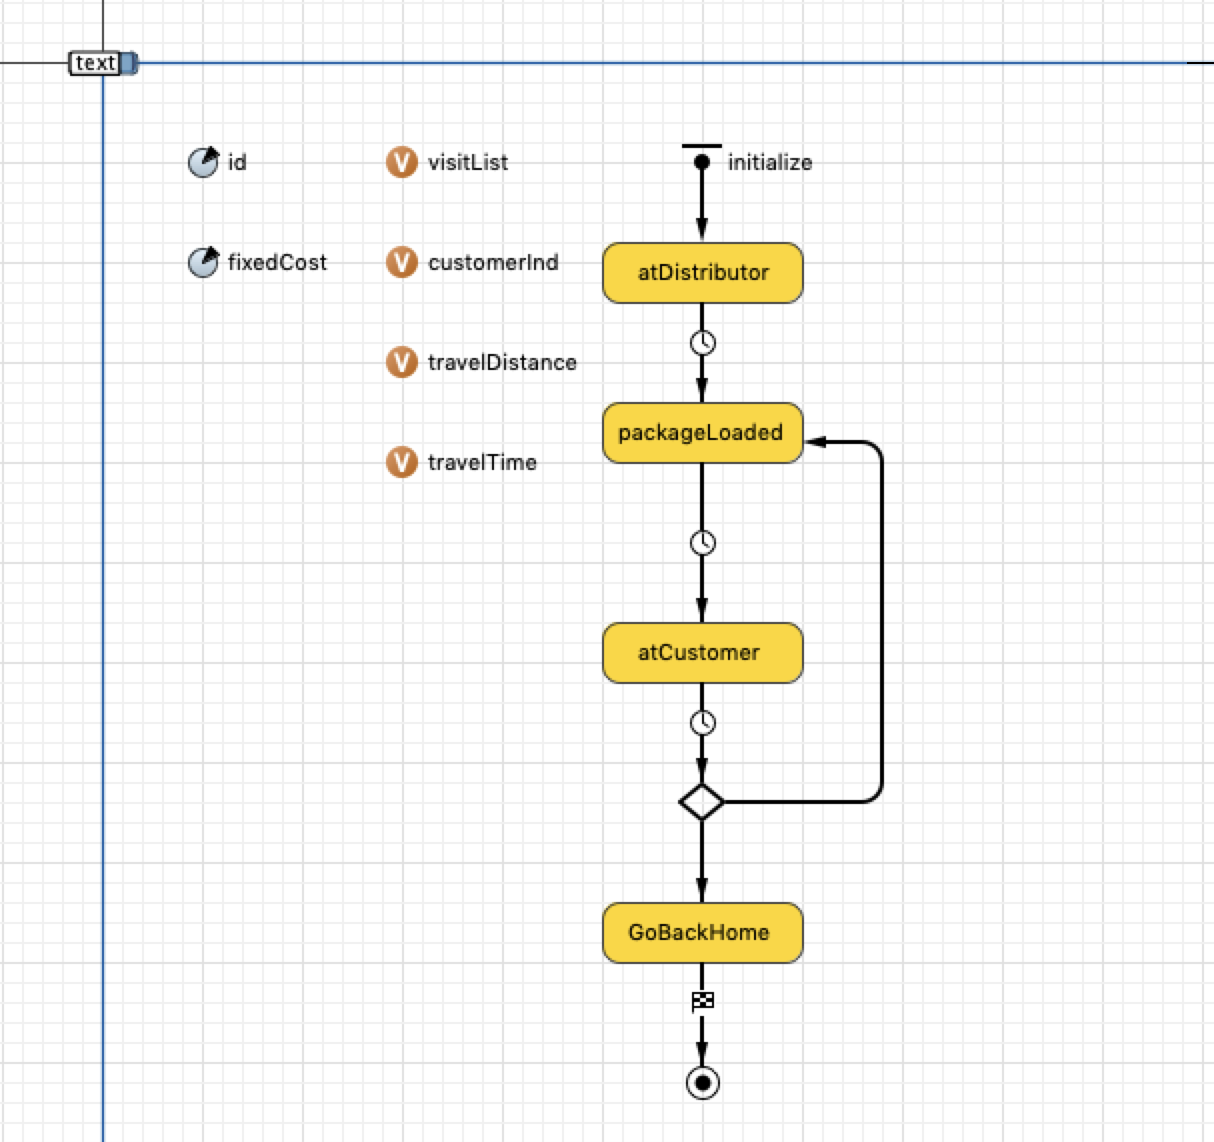
\includegraphics[width=3in]{truck}
	\caption{Agent Truck}
	\end{figure}
	
	\paragraph{}We model this problem as an Agent Based Model (ABM) in AnyLogic. Three datasets are imported into the model: customer sample, distance and time sample and routes of trucks. According to the result in Section 3, Least Distance algorithm gives a better solution. So we used the solutions in Table 6 as our final input. Three types of agents are created, namely Distribution Center, Customer and Truck. Customer has only one parameter called ``id", corresponds to customer ID in our dataset. The construct of Truck is shown in Figure 1. Action codes in each state and transit are listed in Appendix I.
	
	\begin{figure}[htbp]
	\centering 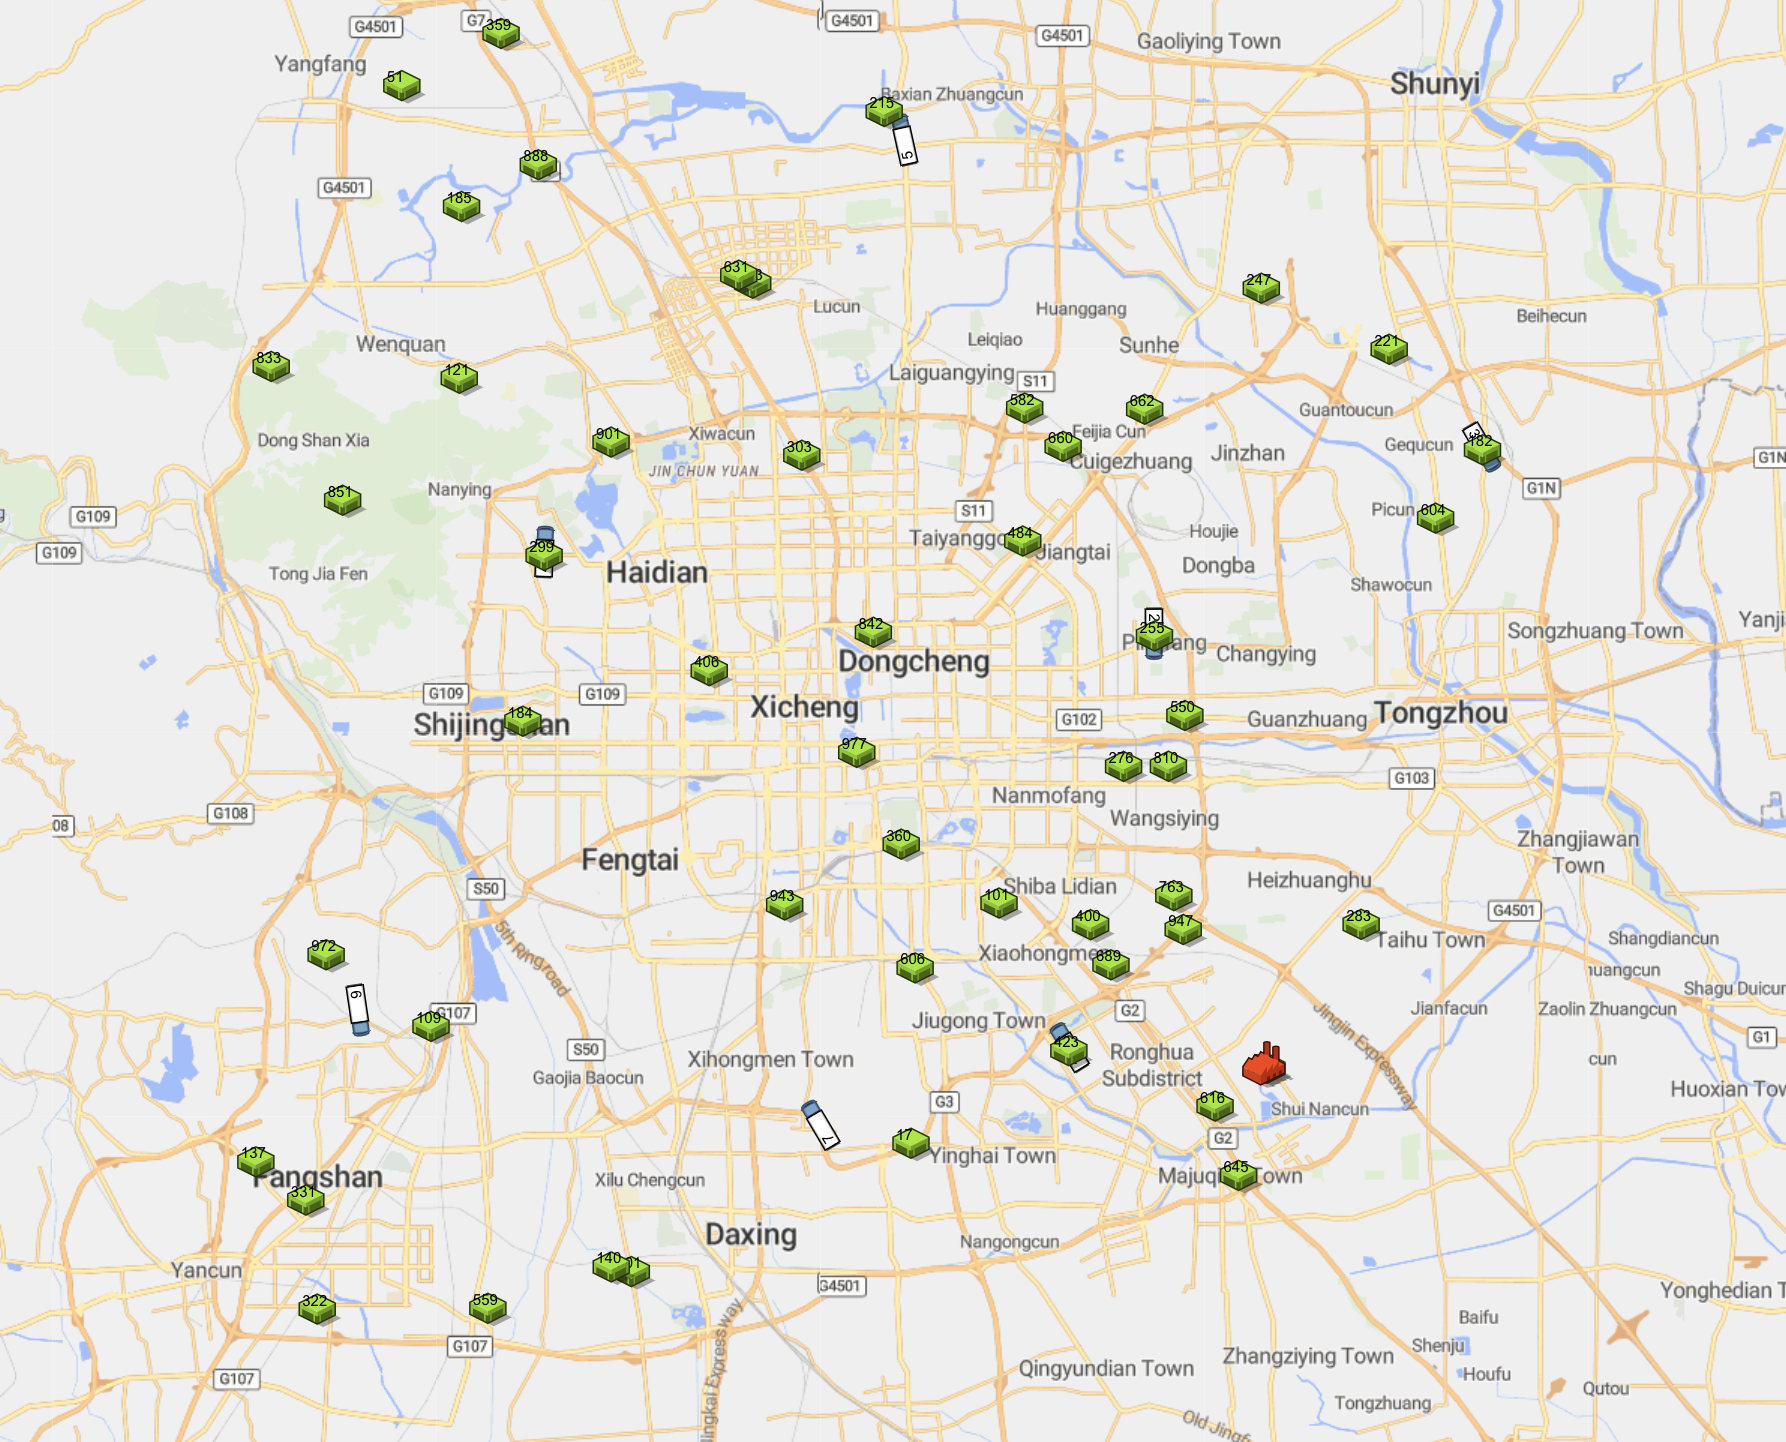
\includegraphics[width=3in]{run}
	\caption{Agent Truck}
	\end{figure}
	
	\paragraph{}To construct the main model, we add customers to a real-world GIS map provided by AnyLogic, using longitude and latitude data from dataset. Trucks and the distribution center are also added to the map based on their coordinates. Trucks are defaulted at the same location with the distribution center and will return to the same location after all packages are delivered. Figure 2 shows one moment of the model running.
	


%Conclusion
\section{Conclusion}

	\paragraph{}In this report, we considered a vehicle routing problem with time windows. A mixed integer program is proposed to solve the model exactly, together with two heuristics algorithm that solve this problem approximately but fast. Comparisons are made according to the results of different algorithms and the results of Least Distance algorithm is finally adopted. Based this, a simulation model is build to visualize vehicle movements around the city.
	
	\paragraph{}Still, a few future works can be done. On one hand, algorithm is very crucial in vehicle routing problem. In our research, we simplify the model because we can not design an algorithm which can solve this problem in an acceptable time. Thus, seeking more effective algorithm could be our future research area. On the other hand, VRP could be extended by adding constraints, such as heterogeneous fleet and multiply trips, etc. Besides,  as electric vehicle get more and more popular because of its economic and environment-friendly advantages, studying when and where to get vehicle recharged are also challenge but meaningful problems.
	
\newpage

% References
\printbibliography

\newpage
% Appendix
\appendix

\section*{Appendix I: Action Codes}

\paragraph{}In the state ``atDistributor":
	\begin{verbatim}
	this.visitList[0] = selectFrom(route).
	where(route.id.eq(this.id)).
	uniqueResult(route.node_1);
this.visitList[1] = selectFrom(route).
	where(route.id.eq(this.id)).
	uniqueResult(route.node_2);
this.visitList[2] = selectFrom(route).
	where(route.id.eq(this.id)).
	uniqueResult(route.node_3);
this.visitList[3] = selectFrom(route).
	where(route.id.eq(this.id)).
	uniqueResult(route.node_4);
this.visitList[4] = selectFrom(route).
	where(route.id.eq(this.id)).
	uniqueResult(route.node_5);
this.visitList[5] = selectFrom(route).
	where(route.id.eq(this.id)).
	uniqueResult(route.node_6);
this.visitList[6] = selectFrom(route).
	where(route.id.eq(this.id)).
	uniqueResult(route.node_7);
this.visitList[7] = selectFrom(route).
	where(route.id.eq(this.id)).
	uniqueResult(route.node_8);
this.visitList[8] = selectFrom(route).
	where(route.id.eq(this.id)).
	uniqueResult(route.node_9);
this.visitList[9] = selectFrom(route).
	where(route.id.eq(this.id)).
	uniqueResult(route.node_10);
this.visitList[10] = selectFrom(route).
	where(route.id.eq(this.id)).
	uniqueResult(route.node_11);
this.visitList[11] = selectFrom(route).
	where(route.id.eq(this.id)).
	uniqueResult(route.node_12);
traceln(this.visitList);
	\end{verbatim}
	
	\paragraph{}In the state ``packageLoaded":
	\begin{verbatim}
	this.travelTime = 60 * selectFrom(dist_time_sample).
	where(dist_time_sample.from_node.eq(visitList[customerInd]),
		  dist_time_sample.to_node.eq(visitList[customerInd + 1])).
	uniqueResult(dist_time_sample.travel_time);
	\end{verbatim}
	
	\paragraph{}In the transit between ``packageLoaded" and ``atCustomer":
	\begin{verbatim}
	moveToInTime(findFirst(main.customers,
	c -> c.id == visitList[customerInd]),
	this.travelTime);
	this.travelDistance = this.travelDistance + 
	selectFrom(dist_time_sample).
	where(dist_time_sample.from_node.eq(visitList[customerInd]),
		  dist_time_sample.to_node.eq(visitList[customerInd + 1])).
	uniqueResult(dist_time_sample.distance);
	\end{verbatim}
	



	
%\end{comment}

\end{document}

%\begin{figure}[htbp]
%\centering \includegraphics[width=4in]{graphs/fig1}
%\caption{Roman Empire and its eight provinces}
%\end{figure}	

%Matrix
%\begin{equation*}
%	\begin{aligned}
%	A_{m\times m}=\left[
%		\begin{array}{ccc}
%			a_{11} & \cdots & a_{1m} \\
%			\vdots & \ddots & \vdots \\
%			a_{m1} & \cdots & a_{mm}\\
%		\end{array}
%		\right],
%	\end{aligned}
%	\end{equation*}





















